% fixture: templates/corpus-slides-default
% oracle: pdflatex
% files: plot.png
% specials: compare
% tier: T3
% engine: document
% covers: the starter-corpus default-theme slides (corpus/slides-default.tex): title page, \tableofcontents, a display and itemize, block and alertblock with inline math, \column columns with align*, a centered \includegraphics of the real plot.png at 0.7\textwidth, enumerate items with overlay specifications
% issue: #361
\documentclass{beamer}
\usepackage{graphicx}
\usepackage{amsmath}

\title{Gradient Descent and Its Variants}
\subtitle{Reading Group, Week 3}
\author{Noah Fischer}
\institute{Machine Learning Lab}
\date{October 2026}

\begin{document}

\begin{frame}
  \titlepage
\end{frame}

\begin{frame}{Outline}
  \tableofcontents
\end{frame}

\section{Basics}
\begin{frame}{The update rule}
  Given a loss $L(\theta)$, gradient descent iterates
  \[
    \theta_{t+1} = \theta_t - \eta \nabla L(\theta_t).
  \]
  \begin{itemize}
    \item $\eta$ is the learning rate.
    \item Too large: divergence. Too small: slow progress.
  \end{itemize}
\end{frame}

\begin{frame}{Convergence}
  \begin{block}{Theorem}
    If $L$ is convex and $\beta$-smooth and $\eta \le 1/\beta$, then
    $L(\theta_T) - L^\star \le \frac{\|\theta_0-\theta^\star\|^2}{2\eta T}$.
  \end{block}
  \begin{alertblock}{Caveat}
    Neural network losses are not convex.
  \end{alertblock}
\end{frame}

\section{Variants}
\begin{frame}{Momentum and Adam}
  \begin{columns}
    \column{0.5\textwidth}
    \textbf{Momentum}
    \begin{align*}
      v_{t+1} &= \mu v_t - \eta \nabla L\\
      \theta_{t+1} &= \theta_t + v_{t+1}
    \end{align*}
    \column{0.5\textwidth}
    \textbf{Adam}
    \begin{itemize}
      \item running mean of gradients
      \item running mean of squares
      \item bias correction
    \end{itemize}
  \end{columns}
\end{frame}

\begin{frame}{Loss curves}
  \centering
  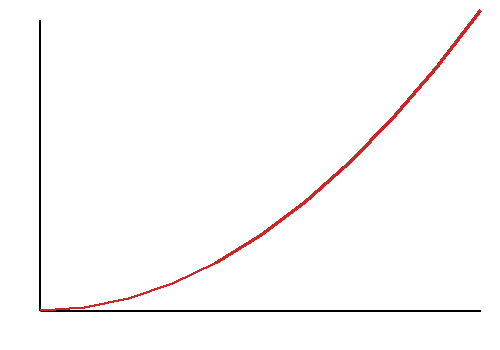
\includegraphics[width=0.7\textwidth]{plot.png}
\end{frame}

\begin{frame}{Takeaways}
  \begin{enumerate}
    \item<1-> Tune the learning rate first.
    \item<2-> Use momentum or Adam by default.
    \item<3-> Schedule the learning rate.
  \end{enumerate}
\end{frame}

\end{document}
